%TODO:
% Background
% General Sentiment Analysis
% add general sentiment analysis to the results
% Conclusions
% author


%  (modified by George Kachergis from Michael Weeks' example_final_report2.tex)
\documentclass[final]{ieee}
\usepackage{graphics}
\usepackage{tabularx}
\journal{CCMLWI}

\title[Cognitive Computational Modeling of Language and Web Interaction]{Bias in Newspaper Headlines}
\author[Br\^{i}ncoveanu \& van Niedek]{%
   Constantin Br\^{i}ncoveanu \\
   Timo van Niedek
    \authorinfo{%
     Cognitive Computational Modeling of Language and Web Interaction,\\
      SOW-MKI61-2016-SEM2-V, 13th July 2017, Dr. G.E. Kachergis. \\
      email: \mbox{c.brincoveanu@student.ru.nl},\mbox{timo.niedek@student.ru.nl}} 
}

\begin{document}

\maketitle

\begin{abstract}
The aim of this project is to detect bias in newspaper headlines using machine learning. A dataset containing world news headlines was obtained using the Reddit API. Bias detection was achieved using several approaches. Firstly, Sentiment Analysis was applied on the headlines. Mean sentiment values can provide information about possible biases. Topic Detection was performed to categorize the headlines, and then Sentiment Analysis was performed on those topic classes, as well as Flavor Analysis. Statistical tests yielded significant biases for a few domains. Lastly, we employed domain classification to gain a different perspective on the biases.
%The abstract should be no more than 150 words.
%It is a short summary of the paper. If you had to
%re-state what your paper says in 150 words or less, what would you
%say? By the way, I recommend writing the abstract LAST, since it is
 %    easier this way.
%      For a conference paper, most people will read the abstract to see
 %     if they find it interesting enough to read the whole paper. This
  %    makes a lot of sense if you go to a conference in a topic that
  %    interests you, but find that there are 100+ other papers.
\end{abstract}

\section{Introduction}\label{sec:intro}

Although newspapers tend to claim neutrality, it is almost impossible to find a source that does not contain any stereotypes or biases in some form. Biases in news headlines pose a danger because they can propagate stereotypes to the general public. The uninterested or time-pressed reader will skim the headlines of newspaper articles or online news collections, often missing important nuances. It is therefore important to be able to detect biased language not only in the body of a news article, but also in the headline by itself. An automatic bias detection system could help guide readers, and expose the hidden biases that are present in news headlines.

Detecting biases manually requires an enormous amount of effort to code news headlines and apply theoretical bias frameworks. It is infeasible to apply this process to the vast amounts of news stories that are released every day. An alternative approach that has gained interest recently is to detect biases automatically using machine learning techniques. These systems employ natural language processing techniques to detect one of the many ways in which bias can be present in texts. One such method is sentiment analysis, in which the polarity of the text is determined, either positive, negative or neutral. Sentiment analysis is typically applied to highly subjective texts for which the polarity is very clear and has high variance across difference texts. The difficulty with using sentiment analysis on news headlines to detect bias is that the polarity scores lie closely together, and therefore do not clearly indicate a bias on its own. News outlets report negative events such as war, death or protests more often than positive events, which makes it difficult to compare polarity scores. Additionally, bias detection using polarity as a measure is not enough since negative scores appear often, even unbiased reports. We therefore propose a technique that investigates the difference between the headline sentiment and the mean of the polarity scores for a specific topic. 

Another method of investigating news bias is to measure the amount of flavor words used by a specific news source. These flavor words are adjectives, adverbs, comparatives and superlatives. The motivation behind this method is that these words can carry bias, and a truly objective report would need less of them. Our method compares the amount of flavor in a headline with the mean of the flavor across one topic to identify which news sources use significantly more flavor as an indicator of bias. 

Our third and final approach is to classify news headlines into their respective sources, which will indicate how distinct a news source is. An unbiased news outlet would be very difficult to classify, whereas a news outlet that consistently uses biased language can easily be classified.

Our methods can be applied in real-world, on-line settings as a tool to make readers aware of the presence of bias. Creating awareness is an important first step in preventing the reinforcement and spreading of unwanted stereotypes. Our proposed methods are applicable to topics and news sources of any kind.

The rest of this paper is structured as follows. In Section \ref{sec:background} we provide an overview of related work, as well as giving the definition of bias that we used to define our work. Section \ref{sec:project} describes the technical details of our work, where Section \ref{sec:project}.\ref{sec:method} describes the methods that we used to detect bias and Section \ref{sec:project}.\ref{sec:evaluation} details how we validated the performance of our techniques. We provide the results in Section \ref{sec:results} and conclude with Section \ref{sec:conclusions}. 

%     The introduction should get the reader interested, explain your
 %    motivations, and provide a quick guide to the rest of the paper.
     
 %     Why is your topic important? Convince us!
 %     Where is it used? What are the applications.
  %    What will you talk about, and what did you do?

  %   Include an overview of the rest of your paper (e.g., section 2
     %       covers...section 3 presents...).
            
            
\section{Background}\label{sec:background}



Most of our computations took a few minutes or less. Topic Detection was the most computationally expensive task, taking a few hours. Our computations were performed on standard laptops.

\subsection{Definition of Bias}\label{sec:definition}
To begin our work, we had to find a good definition for bias. One source\cite{Caverni90} states:
  \begin{quotation}
    "Bias in cognitive science is generally defined as a deviation from a norm, deviation from some true or objective value."
  \end{quotation}
We came up with several ways to detect those deviations from a norm, as will be discussed in the following sections.

%TODO

% Include any relevant and specific info,
 %e.g. hardware statistics, equipment used.
% There is {\bf always} some background to cover.
%            
%           Describe what other people had to say on this topic(s)
%            (be sure to cite your references, and quote as appropriate).
%           Describe what other people did on this topic (or related topics).
%           In the references section, cite the papers/books that you used.
%Talk about problems and shortcomings of their work.
%Talk about how your work is different and better.
%
%Here are some citation examples. 
%This is a book about VLSI \cite{Weste93}.
%Also, the references contain a good conference paper \cite{LiY88},
%and a good journal article \cite{BiS92}.
%Anything you found useful.
%Include textbooks from class if you want.


\section{Project}\label{sec:project}

Our project consists of several approaches which let us detect biases and analyze newspapers from different perspectives. In this section, we are going to provide information about the dataset we used, as well as describe our approaches, ranging from general sentiment analysis, topic detection and sentiment and flavor analysis for the specific topics, to domain classification.

\subsection{Data}

Firstly, we looked at the Kaggle News Aggregator Dataset\cite{Lichman13}. The advantage of this dataset is that it contains over 400k news stories from many different domains. Often, the same event exists in the dataset multiple times, covered by different news sources.
This dataset did not fulfill our requirements, because it only covered a quite small timespan in 2014 and it had a limited number of content categories, and no politic content.

Therefore, we started looking for alternative datasets, which led us to the discovery of the Reddit API. We selected newspaper headlines from "r/worldnews", which exhibits roughly 90k headlines per year. Each headline was obtained with a corresponding timestamp and the domain on which the news story was published. One drawback of our dataset is the fact that each event was usually featured only once in our dataset. If the same event would exist in the dataset several times, covered by different domains, a direct comparison between those domains would have been much easier. We scraped headlines starting from 2014, but for our analysis we mostly focused on the timespan between 2016 and 2017, since the full dataset would make Topic Detection too computationally expensive. Furthermore, the number of topics would probably increase, and some topics would only occur during a short timespan.

Since many domains in the dataset only occurred a few times, and the number of headlines per domain would be further reduced because of the Topic Detection, we selected the big domains to make sure that at least a few hundred headlines per domain were available.

\subsection{Method}\label{sec:method}

%Describe your approach to the problem.
%Describe what you did.
%            What you already had (and where it came from).
%            What you added/changed.
%            For parts, include close-up drawings (e.g. Magic screenshots).

We employed several methods to detect biases. As a first glance at a possible bias, we used Sentiment Analysis. Later, we decided to refine our results by utilizing Topic Detection, Flavor Analysis, as well as a domain classifier.

\subsubsection{General Sentiment Analysis}

% Note: in this section, there shouldn't be any results or discussion, we will add that in the Results & Summary sections
% This section is only for describing the methods
One of our first results was a general Sentiment Analysis. %TODO: explain how it works and how we used it etc.
We aggregated the results by averaging the sentiments of the headlines for each domain. Those average values ranged from $-0.3$ to $-0.1$. %TODO: insert exact values, and maybe also add statistically significance tests.
This revealed some interesting differences between the domains. It became clear that some domains had very negative average sentiments, because they focused on negative topics such as war and general world news, whereas others have relatively positive average sentiments, because they focused on economics or science news. %TODO: add examples and talk more about it
%TODO: add results in Results section

\subsubsection{Topic Detection}

As a more fine-grained measure of bias, we use sentiment analysis per topic. To extract the topics from our data set, we use the biterm topic model (BTM) \cite{BTM13}, which is especially suitable for short texts. BTM uses the word co-occurrence patterns (biterms) to create a model over the entire corpus, thus solving the problem of sparse word co-occurrences within one document. The model parameters are estimated using Gibbs sampling. We create a vocabulary of the top 5000 most occurring words in the corpus, and run the Gibbs sampling algorithm to model $T = 20$ topics. For the Dirichlet priors, we use $\alpha = 50/T = 2.5$ as recommended by \cite{FST13} and $\beta = 0.01$ in order to make the topics contain a small number of highly distinct words. Due to limitations in computational power and the large size of the data set, we were limited to 250 iterations of Gibbs sampling, which took approximately nine hours to complete. We use a modified version of the BTM implementation found at \cite{BTM15}.

\subsubsection{Topic Sentiment Analysis}\label{sec:topic sent}

We determine the topic for all the headlines in the 2017 Reddit data set using the maximum topic probability. We extract the headlines for the selected topics in Table \ref{tab:topics} and compute the polarity score for every headline. We use the VADER sentiment analysis framework \cite{VAD14} since it is has been shown to achieve good performance on short social media text. VADER is able to detect the polarity of complicated sentences with human-like accuracy.

For every topic, we take the mean over the polarity scores of all headlines within the topic, which we call the \textit{mean topic sentiment}. We then calculate the mean over the polarity scores within one topic for every news source separately. The difference between the mean sentiment per news source and the mean topic sentiment is an indicator of bias, using the definition of bias given in Section \ref{sec:background}.\ref{sec:definition}.

\subsubsection{Flavor Analysis}\label{sec:flavor}

As an alternative metric, we introduce the concept of flavor. The amount of flavor in a headline is determined by the amount of words that can potentially carry subjectivity, namely adjectives, adverbs, superlative and comparatives. Intuitively, objective records of news events require less flavor words, while flavorful headlines are more likely to contain bias. We determine the flavor words using the part-of-speech tagger from NLTK \cite{NLTK09}. Since longer sentences are more likely to contain flavor words, we define a normalized flavor metric as the number of flavor words, divided by the total number of words in a sentence.

Similar to the topic sentiment analysis, we compare the flavor per news source and topic with the average flavor taken over all headlines in one topic, the \textit{mean topic flavor}. It is important to note that a deviation from the mean topic flavor does not indicate that a news source is negatively or positively biased for one topic. Instead, such a deviation means that a news source uses significantly more subjective words than others, which we consider an indicator of bias using the definition in Section \ref{sec:intro}.\textit{\ref{sec:definition}}. 

\subsubsection{Domain Classification}
We implemented a Bag of Words model with a Random Forest Classifier to detect the domain for a given headline. For this task, we handpicked six domains. Those were the five most occurring domains: BBC, CNN, Independent, Reuters, and The Guardian. We additionally selected Foxnews as a sixth domain, hoping for it to be a contrast to the other five ones. The number of headlines per domain varies a lot, ranging from just 1,418 headlines (Foxnews) to over 11,000 headlines (BBC). Due to this big imbalance, we applied undersampling to create a balanced dataset, containing 8,508 total headlines. Then we split the data into a training set (80\%) and a test set (20\%).

The Bag of Words model was created by firstly removing stopwords from the headlines and then transforming them into vectors with maximum 5000 features, using a CountVectorizer. Secondly, a Random Forest Classifier was used to predict the domain for the headlines. We found, by trial and error, that 50 is a good number estimators for this task.

\subsection{Evaluation}\label{sec:evaluation}

In this section, we will describe the evaluation metrics used to validate our systems. Since there is no good quantitative measure to evaluate the quality of the detected topics, we instead validated them using a small-scale study in which three participants were asked to define a topic from the top twenty most distinct keywords as found by the BTM, and give a rating on a scale from 1 to 7 for how coherent the topic was. A large-scale study was beyond the scope of this project due to time limitations. We selected a subset of the twenty topics based on average coherence rating and potential for controversy to perform sentiment analysis over. The selected topics can be found in Table \ref{tab:topics}. After extraction of these selected topics, the data set was severely reduced in size. The distribution of headlines per topic is shown in Fig. \ref{fig:topic_dist}, the number of headlines per news source after selecting topics is shown in Fig. \ref{fig:domain_dist}.

\begin{figure}[!hbt]
  
  \centering
    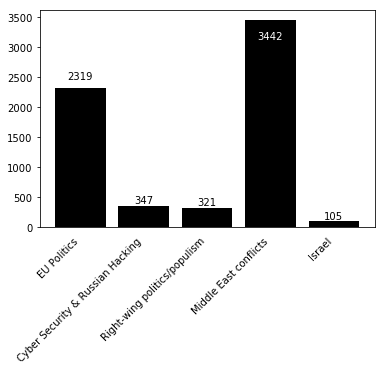
\includegraphics[width=\columnwidth]{topic_dist_bars.png}
    \caption{Number of headlines per topic.}
  \label{fig:topic_dist}
\end{figure}

\begin{figure}[!hbt]
  
  \centering
    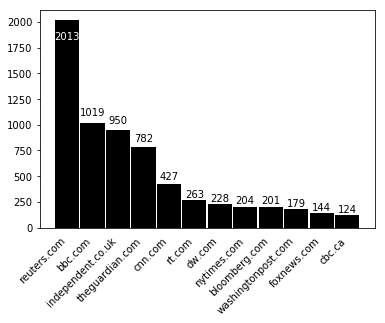
\includegraphics[width=\columnwidth]{domain_dist.png}
    \caption{Number of headlines per news source.}
  \label{fig:domain_dist}
\end{figure}

We validated the per-topic sentiment and flavor analysis using a two-sided paired T-test. For every news source, the measurements were tested against the rest of the population excluding the news source. We did not assume homogeneity of variance across samples. The results of these tests will be shown in Section \ref{sec:results}.

We evaluated the classifier by taking its F1-Score into account, but also looking at other influencial factors, such as the number of classes. A confusion matrix (see Fig. \ref{fig:classificationConfusionMatrix}) helped us to detect domains which were identical to others. For example, \texttt{bbc.co.uk} was often confused with \texttt{bbc.com}. Since headlines of both of those domains come from BBC, we aggregated them into a single class. The same was done for Reuters, CNN and The Guardian. Furthermore, we eliminated domains that regularly post headlines that came from other domains. One example for that is \texttt{yahoo.com}, which takes news stories from various sources and publishes them on their domain. The classification revealed those sources accordingly.

\section{Results}\label{sec:results}

%{\bf Each team member must submit an individual report.}

%            Include relevant observations, measurements, and statistics.
%            For example, for the VLSI Class: Include statistics such as
%            timing information if available by simulation, or if not,
 %           your own analysis about critical path, delays, and clock
%            cycles. Be sure to include size information: the total size
 %           of the circuit measured (X lambda by Y lambda), and the
 %           transistor count. 

\subsection{Sentiment and Flavor Analysis}

The results of the sentiment analysis described in Section \ref{sec:project}.\ref{sec:topic sent} evaluated using a paired T-test are shown in Fig. \ref{fig:mean_sent}.

%TODO: add more interpretation

\begin{figure}[!hbt]
  
  \centering
    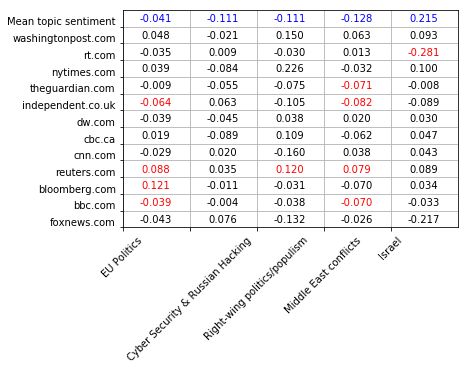
\includegraphics[width=\columnwidth]{mean_sent.png}
    \caption{Deviation from mean topic sentiment per domain. The top row shows the mean topic sentiment in blue. Significant results with $p < 0.05$ are shown in red.}
  \label{fig:mean_sent}
\end{figure}

\begin{figure}[!hbt]
  
  \centering
    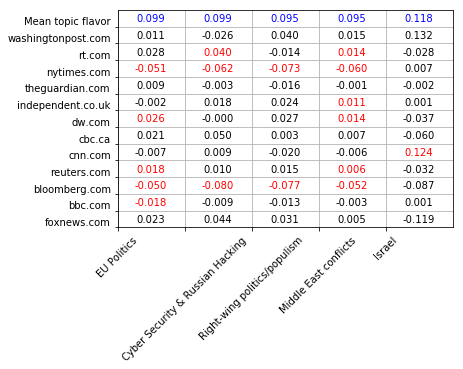
\includegraphics[width=\columnwidth]{mean_flavor.png}
    \caption{Deviation from mean topic flavor per domain. The top row shows the mean topic flavor in blue. Significant results with $p < 0.05$ are shown in red.}
  \label{fig:mean_flavor}
\end{figure}

\subsection{Domain Classification}

The domain classification for our six selected domains yielded an F1-Score of around $0.4842$. The confusion matrix for the classification is shown in Fig. \ref{fig:classificationConfusionMatrix}.

Additionally, we took a look at the feature importances and we examined the words with the highest prediction probabilities for a certain domain. Table \ref{tab:indicativeWords} shows a list of some of the most indicative words.

\begin{figure}[!hbt]
  \centering
    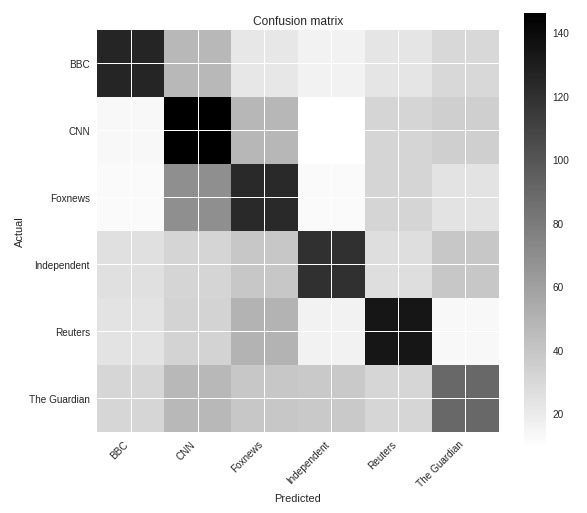
\includegraphics[width=\columnwidth]{classificationConfusionMatrix.png}
    \caption{Confusion matrix for the domain classification.}
  \label{fig:classificationConfusionMatrix}
\end{figure}
            
%\section{Summary}\label{sec:summary}

%TODO: do we need a summary, or maybe it is better to combine it with the Conclusions?

%           Try to draw together the intro, background, and project
 %           sections.
 %          How do they all relate together? (They may appear to be
 %           disjoint sections to an unfamiliar reader).
 %          Restate important results.

\section{Conclusions}\label{sec:conclusions}

We first note that the distribution of sentiment values is informative, since a random distribution would only yield three significant deviations on average. The mean topic sentiment values are negative for all topics except the last topic (``Israel''), which confirms that news reports often yield a negative sentiment value overall. The most interesting result is the large negative relative sentiment value for the topic ``Israel'' for \texttt{rt.com} (Russia Today).

Detecting biases in newspapers is an important task

There are measurable biases in newspaper headlines. Classification yielded surprisingly good results. The detected differences between the respective domains are statistically significant.

Sentiment Analysis is not accurate enough to detect the true sentiment value for each headline. In fact, the individual values often appear disappointingly inaccurate. However, if the number of headlines is big enough, the aggregated mean values per domain show significant differences from the general mean.

There are many more possible approaches to detecting newspaper biases, and we only scratched the surfaces of this broad topic. Further research is definitely going to reveal more.

%           You can combine Summary and Conclusions as you see fit.
%           What was accomplished and learned.
 %          What you would have done differently.
 %          Future work.
           
\begin{thebibliography}{99}
  \bibitem{Lichman13} Lichman, M. (2013). {\it UCI Machine Learning Repository} \texttt{http://archive.ics.uci.edu/ml}. Irvine, CA: University of California, School of Information and Computer Science.

  \bibitem{Caverni90} Caverni J.-P., Fabre J. M., Gonzales, M. (1990): Cognitive biases: their Contribution for Understanding Human Cognitive Processes. Amsterdam: {\it Elsevier Science Publishers B. V.}

  \bibitem{BTM13} Xiaohui Yan, Jiafeng Guo, Yanyan Lan and Xueqi Cheng, 
   ``A Biterm Topic Model for Short Texts'', {\it Proceedings of the 22nd international conference on 
   World Wide Web}, ACM, 2013, pages 1445--1456.

  \bibitem{LDA03} D. M. Blei, A. Y. Ng and M. I. Jordan, ``Latent Dirichlet Allocation'' {\it Journal of machine Learning research},  Jan. (2003), pp.~993--1022.
   
   \bibitem{FST13} Thomas L. Griffiths and Mark Steyvers, 
   ``Finding scientific topics'', {\it Proceedings of the National academy of Sciences}, vol.~101, suppl 1, 2004 pages 5228--5235.
   
   \bibitem{VAD14} Clayton J. Hutto and Eric Gilbert, 
   ``Vader: A parsimonious rule-based model for sentiment analysis of social media text.'', {\it  Eighth international AAAI conference on weblogs and social media}, Ann Arbor, MI, USA, June 2014.
   
   \bibitem{NLTK09} Steven Bird, Ewan Klein and Edward Loper. {\it Natural language processing with Python: analyzing text with the natural language toolkit}, ``O'Reilly Media, Inc.'', 2009.
   
   \bibitem{BTM15} Joan Capdevila Pujol (Universitat Polyt\`{e}cnica de Catalunya), ``jcapde/Biterm: Biterm topic model'', {\it GitHub}, \texttt{https://github.com/jcapde/Biterm}, posted October 14, 2015, accessed May 24, 2017.


  % Book
  %\bibitem{ImABook} Joe Author, {\it Joe's Book About Stuff}, Publisher Press,
  %Atlanta, GA, 2008.
  
  %\bibitem{ImAConfPaper} Jane Scientist and Jake G. Student, 
   %``A Study of Conference Papers'', {\it Proceedings of the 3rd International
    %Conference on Research}, Paris, Texas, USA, January 4-6, 2008, pages 112-115.
    
    %\bibitem{ImAJournalPaper} Jane Scientist, Joe Author, and Jake G. Student,
    %``Journal Papers are Longer than Conference Papers'', 
    %{\it IEEE Transactions on Research}, Volume 4, Number 1, pages 212-235,
    %March 2008.
  
  
  %\bibitem{Weste93} Neil H. E. Weste and Kamran Eshraghian, {\it Principles
  %of CMOS VLSI Design}, 2nd ed. Reading, MA: Addison-Wesley, 1993.

  %Example of a Conference Paper
  %\bibitem{LiY88} R. A. Lincoln and K. Yao, ``Efficient Systolic Kalman
  %Filtering Design by Dependence Graph Mapping,'' in {\it VLSI Signal
  %Processing, III}, IEEE Press, R. W. Brodersen and H. S. Moscovitz Eds.,
  %1988, pp.~396--410.

  % Example of a Journal Paper
  %\bibitem{BiS92} C. H. Bischof and G. M. Shroff, ``On Updating Signal
  %Subspaces,'' {\it IEEE Trans. on Signal Processing}, vol.~40, no.~1,
   %Jan. 1992, pp.~96--105.

  %\bibitem{Lyons97} Richard Lyons, {Understanding Digital Signal Processing},
%Addison-Wesley, 1997.

  %\bibitem{Strang97} Strang and Nguyen, {\it Wavelets and Filter Banks}, Revised
%Edition, Wellesley-Cambridge Press, 1997.

%\bibitem{Weeks99} Michael Weeks, Beth Lumetta, Magdy Bayoumi, "The Black Jack
%Tutor Chip: Dealing From Idea to Silicon," /IEEE Potentials/, April/May
%1999, pages 38-42.

% example conference paper
%\bibitem{Zhang99} Guoqing Zhang, Mike Talley, Wael Badawy, Michael Weeks and
%Magdy Bayoumi, "A Low Power Prototype for a 3-D Discrete Wavelet
%Transform Processor," {\it IEEE International Symposium on Circuits and
%Systems (ISCAS '99)}, Orlando, Florida, May 30-June 2 1999, pages 80-83.



% example webpage
%\bibitem{Clarke04} Peter Clarke (Silicon Strategies), "Silterra demonstrates
%0.13-micron 8-Mbit SRAM", {\it EE Times},
%\texttt{http://www.eetimes.com/semi/news/}
%\texttt{showArticle.jhtml;}
%\texttt{jsessionid=}
%\texttt{0JJT0OEQDLM3MQSNDBGCKH0CJUMEKJVN?}
%\texttt{articleID=54201193},
%posted November 30, 2004 (5:54 AM EST), accessed November 30, 2004.

\end{thebibliography}

\newpage

\hbox{}


\newpage

\thispagestyle{empty}

\onecolumn

\section*{Appendix}

\begin{table}[htb]
\caption{Selected topics within the 2017 Reddit data set}
\begin{tabularx}{\textwidth}{X|l|l}
Keywords & Topic & Average Coherence \\ \hline
election, EU, Brexit, vote, party, president, minister, UK, parliament, presidential, Theresa, May, says, prime, European, Le, Pen, government, would, French & EU Politics & $5.67$ \\ \hline
Russian, Russia, US, intelligence, Trump, hacking, hackers, attack, cyber, CIA, FBI, security, government, former, ex, spy, data, says, officials & Cyber security \& Russian hacking & $6.00$ \\ \hline
Germany, party, Trump, right, says, German, Nazi, world, anti, social, pope, new, election, far, Brexit, leader, president, French, speech, saying & Right-wing politics \& populism & $4.33$ \\ \hline
Syria, Russia, US, north, Korea, Trump, military, missile, UN, war, Israel, turkey, Iran, state, said, Syrian, says, united, forces & Middle East conflicts & $5$ \\ \hline
Israel, Trump, Israeli, president, Netanyahu, house, white, US, Palestinian, Donald, says, minister, Jerusalem, bank, peace, Palestinians, visit, settlements, west, two & Israel & $5.66$ \\
\end{tabularx}
\label{tab:topics}
\end{table}

\begin{table}[htb]
\caption{Most indicative words for the domain classification}
\begin{tabularx}{\textwidth}{X|l|l}
Word & Highest probability & Predicted domain \\ \hline
mosul & 0.94 & CNN \\ \hline
us & 0.84 & CNN \\ \hline
sues & 0.815 & BBC \\ \hline
aleppo & 0.8 & CNN \\ \hline
reportedly & 0.8 & Foxnews \\ \hline
japan & 0.78 & CNN \\ \hline
turns & 0.77 & BBC \\ \hline
investigates & 0.76 & BBC \\ \hline
cnn & 0.76 & CNN \\ \hline
pepe & 0.747 & BBC \\ \hline
cyclone & 0.745 & BBC \\ \hline
bbc & 0.727 & BBC \\ \hline
erdo & 0.725 & The Guardian \\ \hline
billion & 0.72 & Reuters \\ \hline
indonesian & 0.72 & Foxnews \\ \hline
football & 0.718 & BBC \\
\end{tabularx}
\label{tab:indicativeWords}
\end{table}

\end{document}
